\section{Adição de Vetores}

Consideremos os vetores $\mathbf{\overrightarrow{u}}$ e
$\mathbf{\overrightarrow{v}}$, cuja soma $\mathbf{\overrightarrow{u}} +
\mathbf{\overrightarrow{v}}$ queremos encontrar. Escolhemos um ponto $A$ e, com
origem nele, traçamos um segmento orientado $AB$ representando
$\mathbf{\overrightarrow{u}}$. A partir da extremidade $B$, traçamos o segmento
orientado $BC$ representando $\mathbf{v}$. O vetor soma
$\mathbf{\overrightarrow{u}} + \mathbf{\overrightarrow{v}}$ é então representado
pelo segmento orientado de origem $A$ e extremidade $C$ na
Figura~\ref{fig:fig1.14}.

\begin{figure}[H]
    \centering
    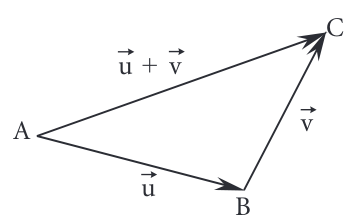
\includegraphics[width=0.3\textwidth]{./fig/fig1.14.png}
    \caption{}\label{fig:fig1.14}
\end{figure}

\[
  \mathbf{\overrightarrow{u}} + \mathbf{\overrightarrow{v}} = \overrightarrow{AB}
  \, \text{ou} \,
  \mathbf{\overrightarrow{AB}} + \mathbf{\overrightarrow{BC}} = \overrightarrow{AC}
\]

Se $\mathbf{\overrightarrow{u}} \parallel \mathbf{\overrightarrow{v}}$, a
obtenção da soma segue o mesmo princípio, ilustrado quando os vetores têm o
mesmo sentido ou sentidos opostos como mostrado na Figura~\ref{fig:fig1.15}.

\begin{figure}[H]
    \centering
    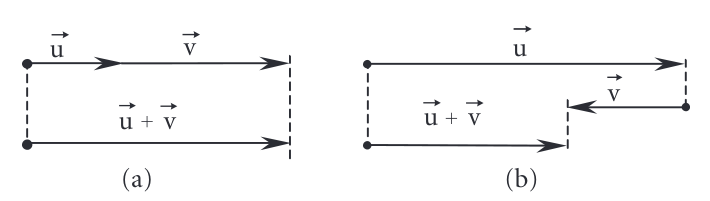
\includegraphics[width=0.7\textwidth]{./fig/fig1.15.png}
    \caption{}\label{fig:fig1.15}
\end{figure}

Caso $\mathbf{\overrightarrow{u}}$ e $\mathbf{\overrightarrow{v}}$ não sejam
paralelos, podemos utilizar o método do paralelogramo. Representamos
$\mathbf{\overrightarrow{u}} = \overrightarrow{AB}$ e
$\mathbf{\overrightarrow{v}} = \overrightarrow{AD}$ a partir da mesma origem
$A$. Construímos o paralelogramo $ABCD$, e o vetor soma
$\mathbf{\overrightarrow{u}} + \mathbf{\overrightarrow{v}}$ é a diagonal de
origem $A$ como vemos na Figura~\ref{fig:fig1.16}.

\begin{figure}[H]
    \centering
    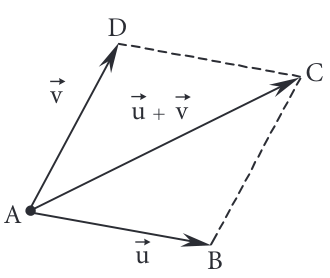
\includegraphics[width=0.3\textwidth]{./fig/fig1.16.png}
    \caption{}\label{fig:fig1.16}
\end{figure}

\[
  \mathbf{\overrightarrow{u}} + \mathbf{\overrightarrow{v}} = \overrightarrow{AC}
  \, \text{ou} \,
  \mathbf{\overrightarrow{AB}} + \mathbf{\overrightarrow{AD}} = \overrightarrow{AC}
\]

Para a soma de três ou mais vetores, o procedimento é análogo. Se a extremidade
do último vetor coincidir com a origem do primeiro, a soma resulta no vetor
  nulo (Figura~\ref{fig:fig1.17}):

\begin{figure}[H]
    \centering
    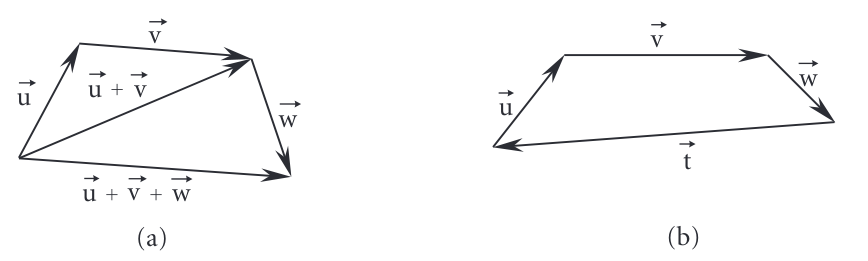
\includegraphics[width=0.7\textwidth]{./fig/fig1.17.png}
    \caption{}\label{fig:fig1.17}
\end{figure}

\[
\mathbf{\overrightarrow{u}} + \mathbf{\overrightarrow{v}} +
\mathbf{\overrightarrow{w}} + \mathbf{\overrightarrow{t}} =
\mathbf{\overrightarrow{0}}.
\]

A adição vetorial possui as seguintes propriedades:

\begin{itemize}
    \item \textbf{Comutativa}: $\mathbf{\overrightarrow{u}} +
      \mathbf{\overrightarrow{v}} = \mathbf{\overrightarrow{v}} +
      \mathbf{\overrightarrow{u}}$.
    \item \textbf{Associativa}: $(\mathbf{\overrightarrow{u}} +
      \mathbf{\overrightarrow{v}}) + \mathbf{\overrightarrow{w}} =
      \mathbf{\overrightarrow{u}} + (\mathbf{\overrightarrow{v}} +
      \mathbf{\overrightarrow{w}})$.
    \item \textbf{Elemento neutro}: $\mathbf{\overrightarrow{u}} +
      \mathbf{\overrightarrow{0}} = \mathbf{\overrightarrow{u}}$.
    \item \textbf{Elemento oposto}: $\mathbf{\overrightarrow{u}} +
      (-\mathbf{\overrightarrow{u}}) = \mathbf{\overrightarrow{0}}$.
\end{itemize}

A diferença entre vetores é definida como:

\[
\mathbf{\overrightarrow{u}} - \mathbf{\overrightarrow{v}} =
\mathbf{\overrightarrow{u}} + (-\mathbf{\overrightarrow{v}}).
\]

No paralelogramo formado por $\mathbf{\overrightarrow{u}}$ e
$\mathbf{\overrightarrow{v}}$, a soma $\mathbf{\overrightarrow{u}} +
\mathbf{\overrightarrow{v}}$ corresponde a uma das diagonais, enquanto a
diferença $\mathbf{\overrightarrow{u}} - \mathbf{\overrightarrow{v}}$ é
representada pela outra diagonal (Figura~\ref{fig:fig1.18}).

\begin{figure}[H]
    \centering
    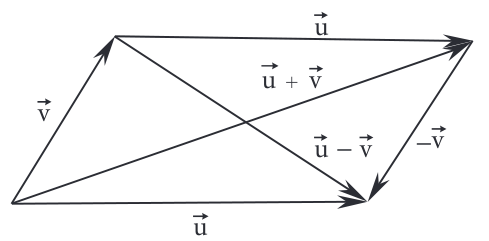
\includegraphics[width=0.35\textwidth]{./fig/fig1.18.png}
    \caption{}\label{fig:fig1.18}
\end{figure}

\newpage

\subsection{Exemplos}

\question{
  Dados dois vetores \( \overrightarrow{u} \) e \( \overrightarrow{v} \) não
  paralelos, construir no mesmo gráfico os vetores  \( \overrightarrow{u} +
  \overrightarrow{v} \), \( \overrightarrow{u} -  \overrightarrow{v} \), \(
  \overrightarrow{v} - \overrightarrow{u} \) e \( -\overrightarrow{u} -
  \overrightarrow{v} \), todos com origem em um mesmo ponto.
}
\answer{
  \begin{figure}[H]
    \centering
    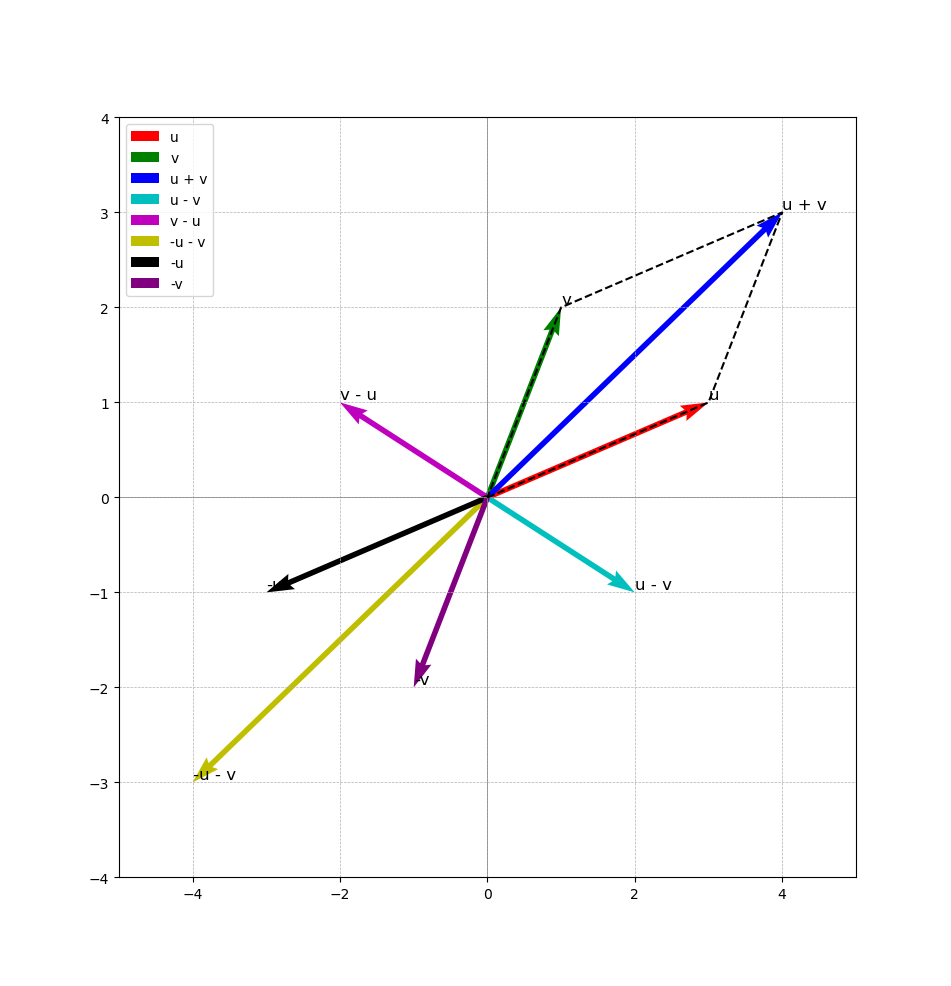
\includegraphics[width=1\textwidth]{./fig/q3.png}
  \end{figure}
}

\newpage

\question{
  Provar que as diagonais de um paralelogramo têm o mesmo ponto médio.
}
\answer{
  \begin{figure}[H]
    \centering
    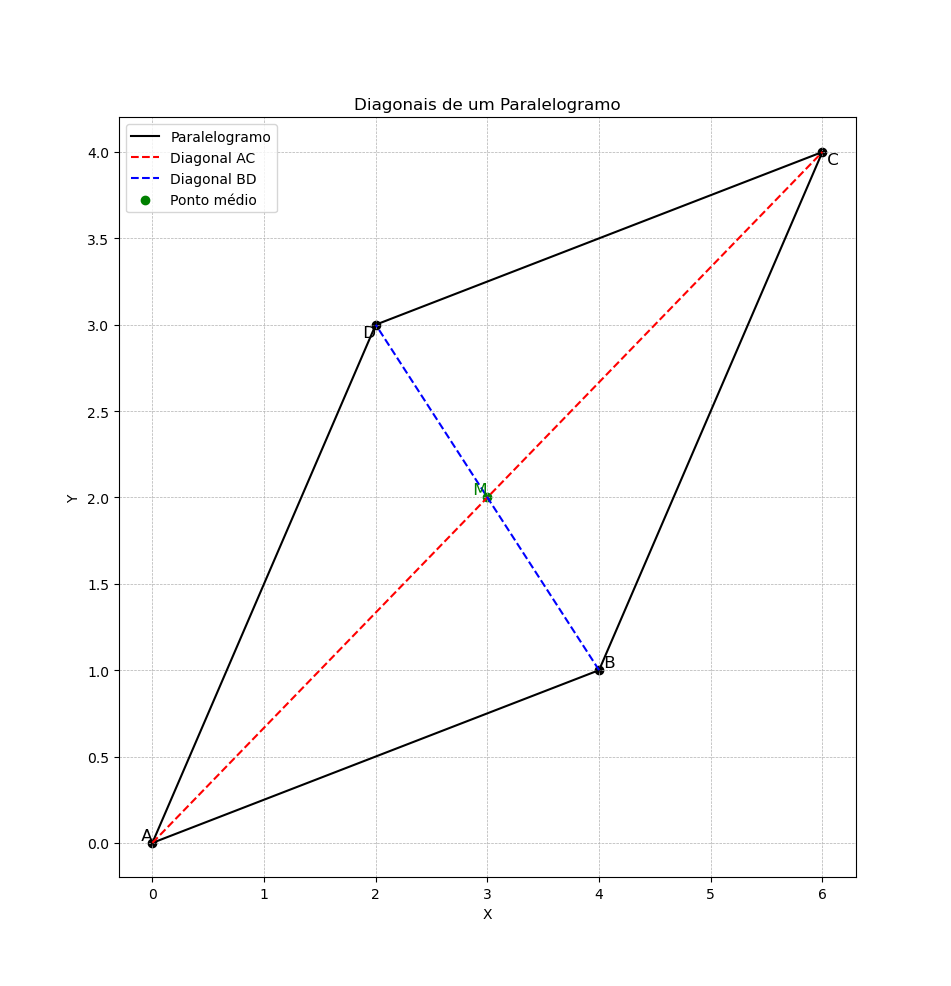
\includegraphics[width=1\textwidth]{./fig/q4.png}
  \end{figure}
  Consideremos o paralelogramo \(ABCD\) de diagonais \(AC\) e \(BD\) e seja
  \(M\) o ponto médio de \(AC\), o que equivale a dizer que 
  \[
    \overrightarrow{AM} = \overrightarrow{MC}.
  \]
  Provemos que \(M\) é também ponto médio de \(BD\):
  \[
    \begin{aligned}
      \overrightarrow{BM} &= \overrightarrow{BC} + \overrightarrow{CM} 
      && \text{(definição de soma)} \\
      &= \overrightarrow{AD} + \overrightarrow{MA} 
      && \text{(igualdade de vetores)} \\
      &= \overrightarrow{MA} + \overrightarrow{AD} 
      && \text{(propriedade comutativa)} \\
      &= \overrightarrow{MD} 
      && \text{(definição de soma)}
    \end{aligned}
  \]
  Como \(\overrightarrow{BM} = \overrightarrow{MD}\), conclui-se que \(M\) é
  ponto médio de \(BD\).
}
